% !TeX encoding = UTF-8
% !TeX spellcheck = <none>

\section{图表}
%%%%%%%%%%%%%%%%%%%%%%%%%%%%%%%%%%%%%%%%%%%%%%%%%%%%%%%
\subsection{插入图片}
\LaTeX支持多种格式的图片,其中包括png、jpg等常见位图,以及pdf、eps等\textbf{矢量图}格式。
矢量图尤其适合科技论文中用于数据展示的各种曲线图和柱状图、饼状图,因为无论如何缩放图像都不会失真。你可以尝试缩放生成的pdf文件到最大,然后观察图~\ref{fig1},图~\ref{fig3}和图\ref{fig:fig3d}中的曲线。

\begin{figure}[!h]
	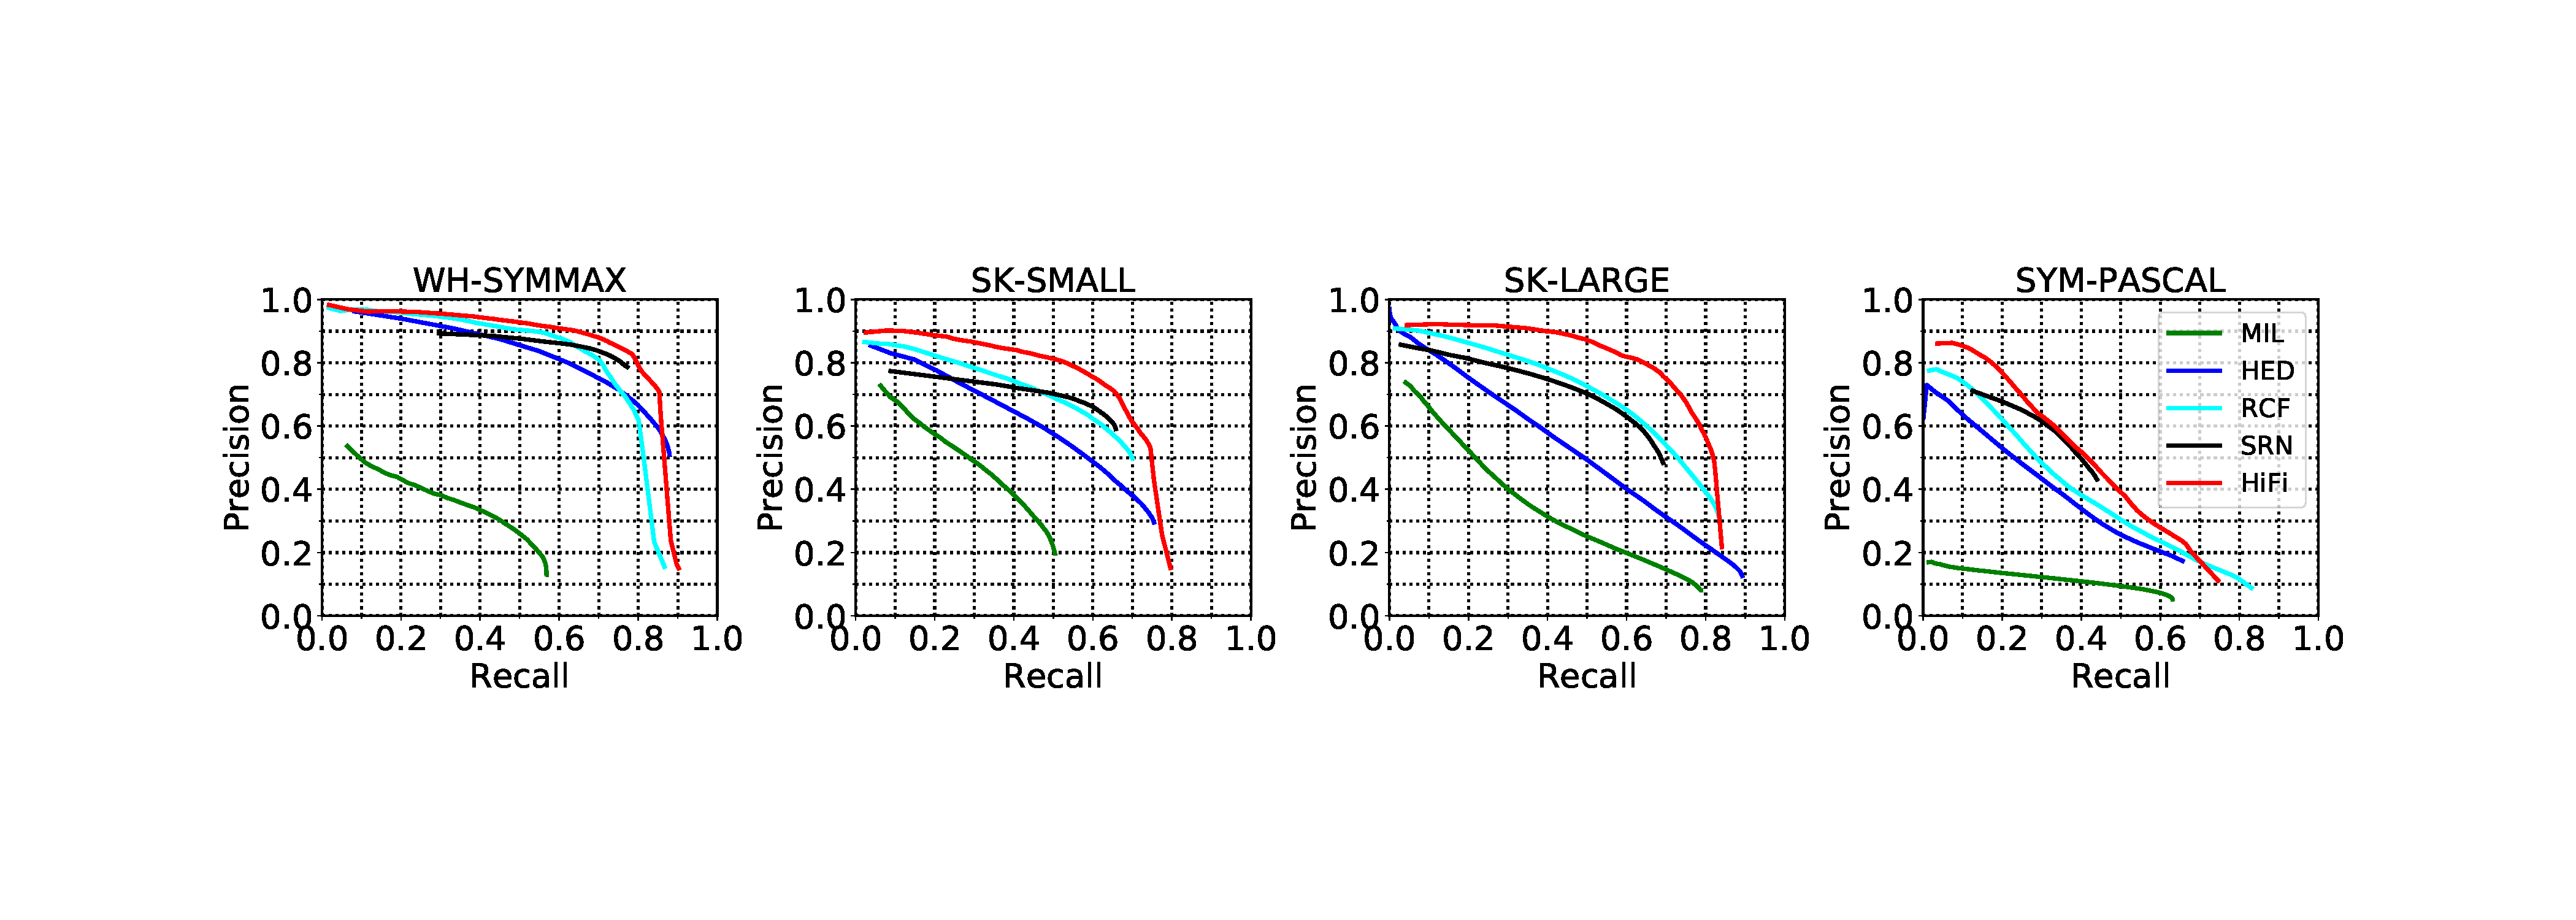
\includegraphics[width=1\linewidth]{figures/pr-curve}
	\caption{一个pdf格式的矢量图。使用\\caption命令为图表添加注解,注解中可以引用参考文献~\cite{shen2017label}。}\label{fig1}
\end{figure}

对于曲线图和柱状图等非照片类图表,我推荐插入pdf格式。pdf格式支持绝大部分主流平台(Windows, Linux, OSX),而且可以方便的自由编辑,文件大小也比较小。
如果你使用Python的Matplotlib画图,那么可以直接用matplotlib.pyplot.savefig()
来导出.pdf格式的图片。
如果你使用Matlab画图的话,只能导出eps格式的矢量图。在\LaTeX中插入eps也没有问题,
但是eps文件比同等条件的pdf稍大,而且不方便编辑。
强迫症患者可以将eps转为pdf后再插入到\LaTeX。

同样是一行四列的布局,图~\ref{fig1}直接插入一个包含四个曲线图的pdf文件,
而图~\ref{fig:fig3d}通过增加一个$1\times4$的表格,然后再每个表格单元中各自插入
一个图标文件。

\begin{figure}[!h]
	\centering
	\begin{overpic}[scale=0.6]{figures/convergence}
		\put(50,41){\large{可使用overpic命令}}
		\put(38, 35){\Large{往图像上覆盖符号$\Sigma$}}
		\put(35,28){\LARGE{公式$f(x)=a\times x$}}
		\put(30,20){\huge{引用公式\ref{eq:cases}。}}
		\put(25,12){\Huge{参考文献\cite{shen2016object}。}}
	\end{overpic}
	\caption{一个pdf格式的矢量图。使用\\caption命令为图表添加注解,注解中可以引用参考文献~\cite{shen2017deepskeleton}。}
	\label{fig3}
\end{figure}

\begin{figure}[!h]
	\centering
	\begin{tabular}{@{}cccc@{}}
		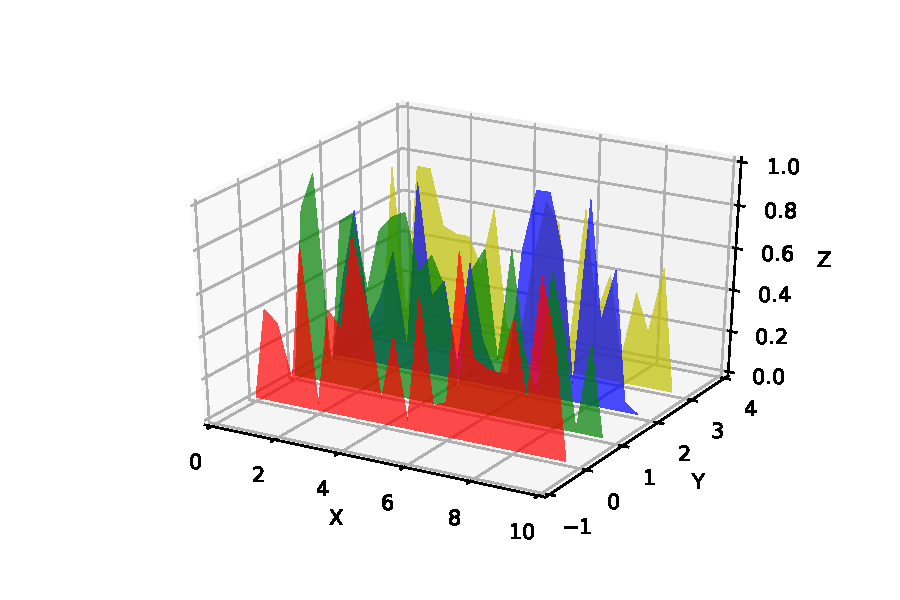
\includegraphics[width=.25\textwidth]{figures/mplot3d}  &
		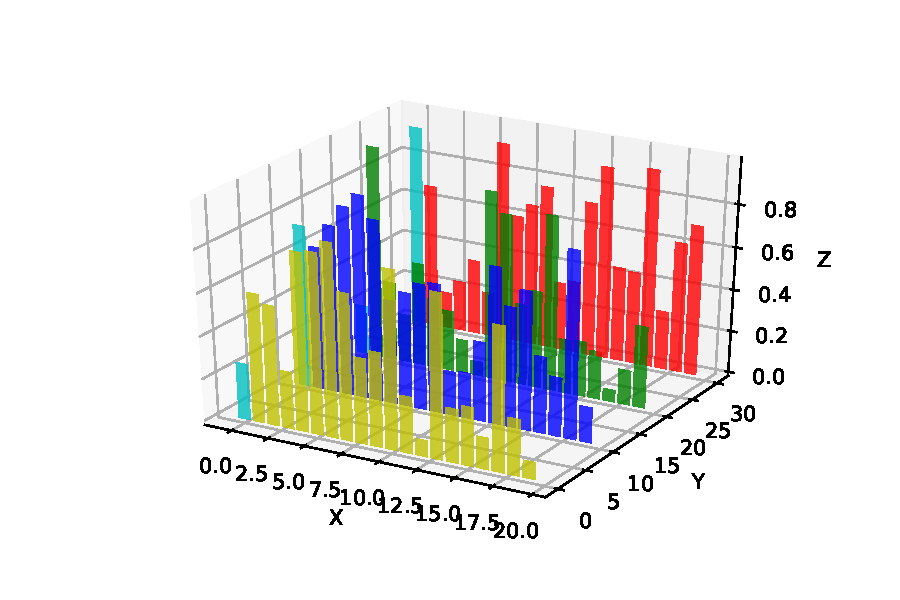
\includegraphics[width=.25\textwidth]{figures/bar3d}  &
		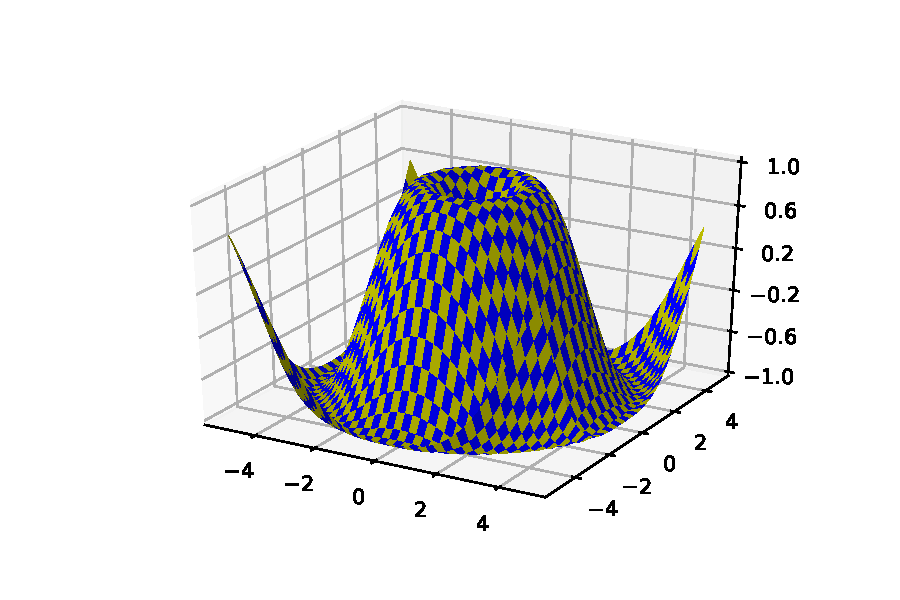
\includegraphics[width=.25\textwidth]{figures/surface3d} &
		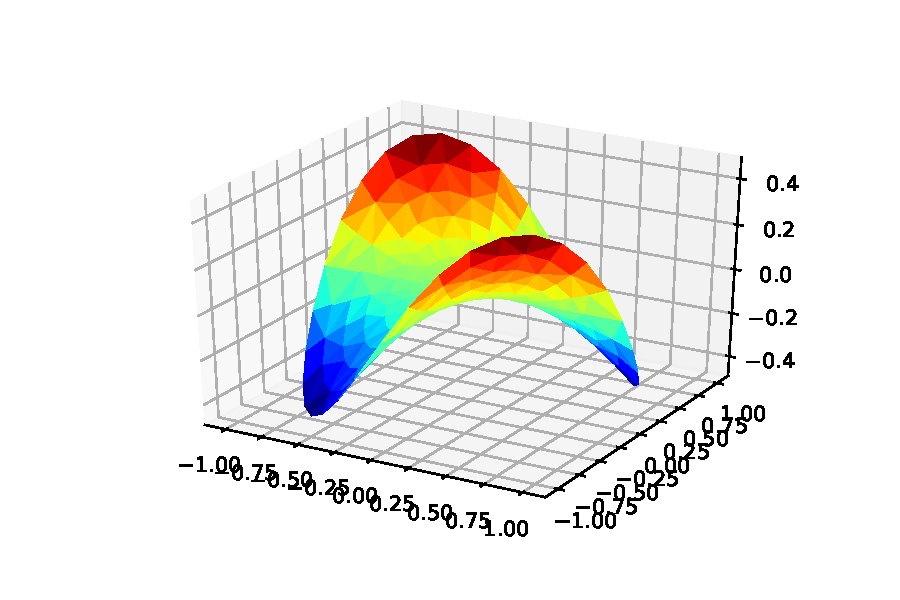
\includegraphics[width=.25\textwidth]{figures/trisurf3d} \\
		(a)M-plot 3D & (b)Bar-chart 3D & 
		(c)Surface 3D & (d) Tri-surface 3D \\
	\end{tabular}
	\caption{通过表格对图片进行布局,在一个$1\times4$表格的每一个单元格中各自插入一个图片文件。
		生成上面四个图对应的Python代码在\href{https://github.com/zeakey/shu-thesis/tree/master/figures}{figures}目录下。}
	\label{fig:fig3d}
\end{figure}
下面是相关代码:
\begin{lstlisting}[captionpos=b,language=Tex]
	\begin{figure}[!h]
		\centering
		\begin{tabular}{@{}cccc@{}}
			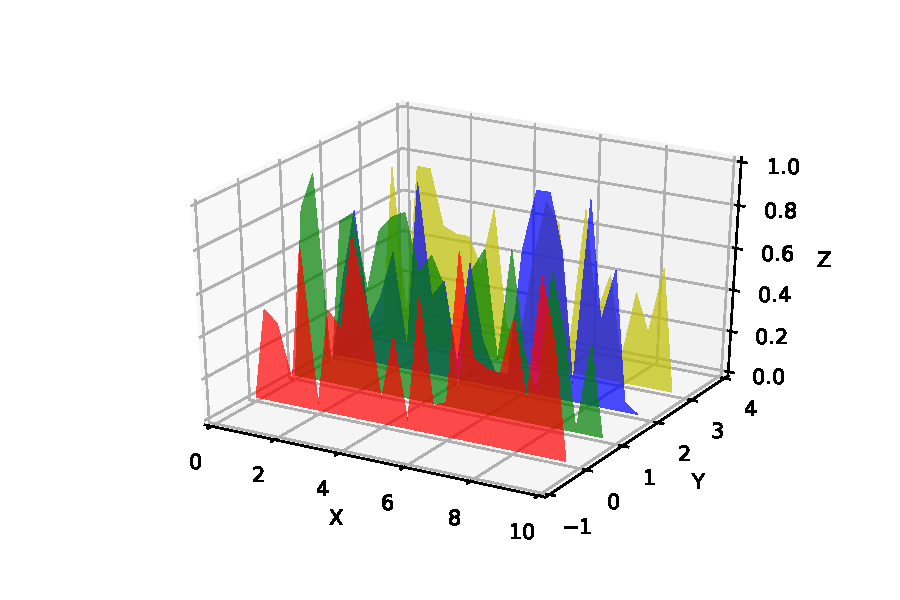
\includegraphics[width=.25\textwidth]{figures/mplot3d}  &
			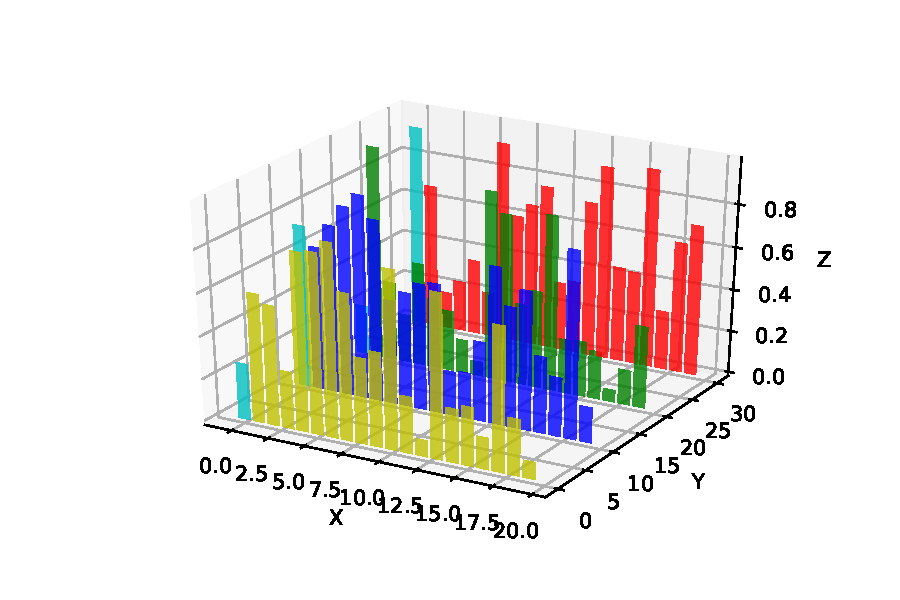
\includegraphics[width=.25\textwidth]{figures/bar3d}  &
			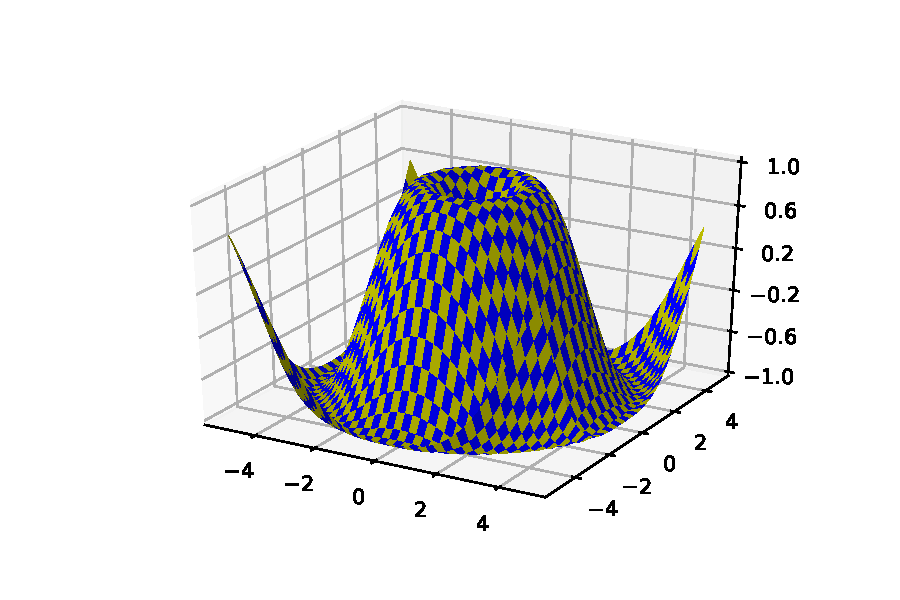
\includegraphics[width=.25\textwidth]{figures/surface3d} &
			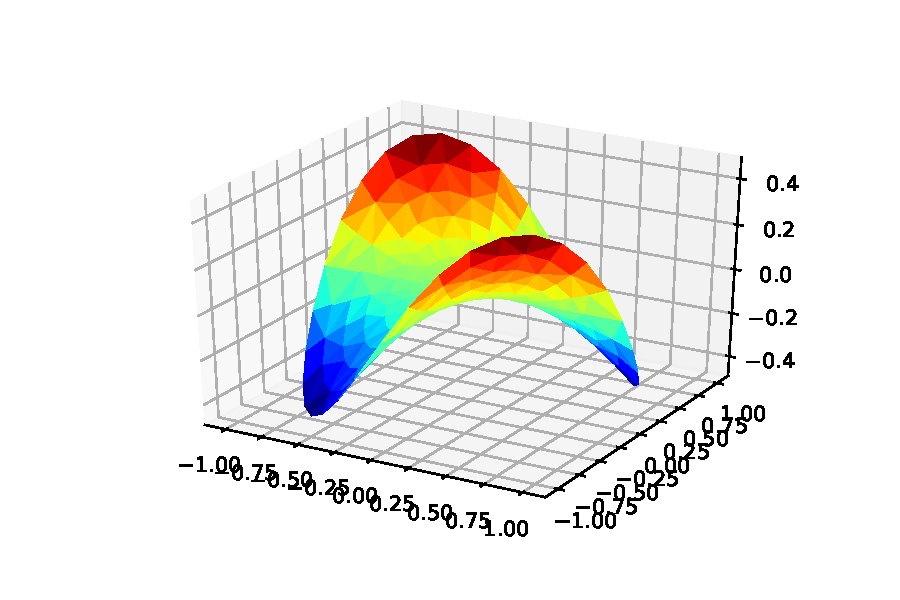
\includegraphics[width=.25\textwidth]{figures/trisurf3d} \\
			(a)M-plot 3D & (b)Bar-chart 3D & 
			(c)Surface 3D & (d) Tri-surface 3D \\
		\end{tabular}
	\end{figure}
\end{lstlisting}

\subsection{绘图}
除了通过直接插入已经生成的图像文件之外,\LaTeX 还可以通过 Tikz 宏包直接绘制函数图像。
%
下面有几个使用Tikz包绘制三位函数曲面和直方图的例子,由于 Tikz 会让编译的时间变长,代码已经被注释。
%
如果你有兴趣的话可以取消注释然后编译查看效果,或者预览预编译的pdf:
\url{http://data.kaiz.xyz/shu-thesis/shu-thesis.pdf}。

%\begin{figure}[!h]
%\centering
%\begin{tabular}{@{}cc@{}}
%  \pgfplotsset{width=0.5\textwidth}
%  \begin{tikzpicture}
	%    \begin{axis}[
		%    hide axis,                              %隐藏坐标
		%    colormap/cool,                          %颜色风格
		%    ]
		%    \addplot3[
		%    mesh,                                   %绘制的三维图像是网格
		%    samples=50,                             %定义域分割数量
		%    domain=-8:8,                            %定义域
		%    ]
		%    {sin(deg(sqrt(x^2+y^2)))/sqrt(x^2+y^2)};    %二元显式函数
		%        \addlegendentry{$\frac{sin(r)}{r}$}         %添加图例
		%    \end{axis}
	%  \end{tikzpicture} & 
%  %==============================%
%  \pgfplotsset{width=0.5\textwidth}
%  \begin{tikzpicture}
	%    \begin{axis}[colorbar]         % 绘制坐标,并设置一个彩色指示条
		%    \addplot3[surf]                % 绘制三维图
		%    {x^2+y^2};                    % 输入二元显式函数
		%    \end{axis}
	%  \end{tikzpicture}
%\end{tabular}
%\caption{通过Tikz绘制函数图像。}
%\label{fig:tikz_surface}
%\end{figure}
%还有直方图:
%\begin{figure}[!hbt]
%\centering
%\pgfplotsset{width=0.5\textwidth}
%\begin{tikzpicture}
%\begin{axis}[ybar,enlargelimits=0.15]  % 绘制关于y坐标的条形图,条形之间的最大间隔是0.15cm
%\addplot[draw=blue,fill=red]           % 蓝色边界、红色填充
%coordinates
%{
	% (0,4) (1,1) (2,2)
	% (3,5) (4,6) (5,1)
	%};
%\addplot[draw=black,fill=blue]         % 黑色边界、蓝色填充
%coordinates
%{
	% (0,3) (1,4) (2,2)
	% (3,9) (4,6) (5,2)
	%};
%\end{axis}
%\end{tikzpicture}
%\caption{通过Tikz绘制直方图。}\label{fig:tikz_hist}
%\end{figure}
%

本章节的所有图像都是\textbf{使用\LaTeX 代码直接绘制的},并没有使用任何Matlab或者matplotlib等第三方程序生成图像。
当然,生成的的图像全部都是矢量图。

%\pagebreak
\subsection{表格}
\LaTeX使用table环境生成表格。下面就是生成表\ref{tab:performance}的\LaTeX代码:

\begin{lstlisting}[captionpos=b,language=Tex]
	\begin{table}[!h]
		\centering
		\setlength\tabcolsep{6.4pt}
		\begin{tabular}{l|c|c|c|c}
			\hline
			\diagbox{Method}{Dataset} & A & B & C & D \\
			\hline
			LMSDS~\cite{shen2017deepskeleton} & 0.365  & 0.392 & 0.293 & 0.174 \\
			LDLF~\cite{shen2017label} & 0.732  & 0.542 & 0.497 & 0.369 \\
			\hline
			\textbf{FSDS} (ours) & 0.769  & 0.623 & 0.633 & 0.418 \\
			\hline
		\end{tabular}\vspace{-6pt}
		\caption{This is a table.}\label{tab:sk-fmeasure}\label{tab:performance}%
	\end{table}%
\end{lstlisting}

\begin{table}[!h]
	\centering
	\setlength\tabcolsep{6.4pt}
	\begin{tabular}{l|c|c|c|c}
		\hline
		\diagbox{Method}{Dataset} & A & B & C & D \\
		\hline
		LMSDS~\cite{shen2017deepskeleton} & 0.365  & 0.392 & 0.293 & 0.174 \\
		LDLF~\cite{shen2017label} & 0.732  & 0.542 & 0.497 & 0.369 \\
		\hline
		\textbf{FSDS} (ours) & 0.769  & 0.623 & 0.633 & 0.418 \\
		\hline
	\end{tabular}\vspace{-6pt}
	\caption{This is a table.}\label{tab:sk-fmeasure}\label{tab:performance}%
\end{table}%

\subsection{图表的排版和定位}\label{sec:location}
\LaTeX相比Word有个缺点就是\emph{非所见即所得}。比如你的两个表格在代码中明明是
相邻一个在前一个在后的,然而排版出来的结果可能是两个被放到了不同的页面中,甚至先后顺序都不对应。
%

\LaTeX图表使用位置参数来确定元素的定位。位置参数有以下几种选项:h (here)、t (top)、b (bottom)、p (我也不知道),分别表示把元素至于当前位置、当前页面的上方、下方。
当你有排版困惑,怎么弄也无法把图标放在自己想要的位置的时候(我经常遇到),最好的解决方法就是疯狂前后移动图表元素对应代码,总有一个位置会是对的。
%
\href{https://tex.stackexchange.com/questions/35125/how-to-use-the-placement-options-t-h-with-figures}{这里}是一个对位置参数的详细介绍。
